\chapter{Entrada/Salida y Archivos}

\section{RAID}

RAID (Vector Redundante de Discos Independientes) es un conjunto de unidades de disco físico vistas por el SO como una sola unidad o volumen lógico.

Con múltiples discos que funcionan en forma independiente y en paralelo, las distintas solicitudes de E/S se pueden gestionar en paralelo siempre que los datos solicitados residan en discos separados. Es más, una única petición de E/S se puede ejecutar en paralelo si el bloque de datos que se pretende acceder está distribuido a lo largo de múltiples discos. Por lo que RAID tiende a mejorar significativamente el rendimiento y/o fiabilidad del sistema de E/S a disco.

\section{Tipos de RAID simples}

A modo de comparación entre tipos de RAID, se utilizará una plantilla con los datos de cada tipo como se muestra en el cuadro \ref{tab:template_raid}. 
\begin{table}[!ht]
  \centering
  \begin{tabular}{l|c}
    Cantidad de discos mínima & N \\\hline
    Cantidad de discos que pueden fallar & M \\ \hline
    Velocidad de escritura relativa a un disco & \(v\)[MB/s] \\\hline
    Velocidad de escritura ponderada & \(w_p\) (1 a 10) \\ \hline
    Velocidad de lectura relativa a un disco & \(v\)[MB/s] \\ \hline
    Velocidad de lectura ponderada & \(r_p\) (1 a 10) \\ \hline
    Costo & Alto/Medio/Bajo
  \end{tabular}
  \caption{Plantilla de comparación entre tipos de RAID.}
  \label{tab:template_raid}
\end{table}

En el cuadro \ref{tab:template_raid} se muestran las velocidades ponderadas \(r_p\) y \(w_p\). Este valor sirve para comparar con respecto a un solo disco. A modo de referencia 5 es el valor de \(r_p\) y \(w_p\) de un solo disco. Un valor más alto indica mayor velocidad y uno más bajo menor.

\subsection{RAID 0}

RAID 0 es una técnica de almacenamiento cuyo objetivo principal es aumentar el rendimiento, no la confiabilidad.

Conceptualmente, RAID 0 divide la información en bloques y distribuye esos bloques entre dos o más discos. En lugar de escribir un archivo completo en un único disco, los bloques se reparten de forma alternada.

Por ejemplo, si un archivo se divide en diez bloques, se reparten entre dos discos como se muestra en la figura \ref{fig:raid0}.

\begin{figure}[!ht]
  \centering
  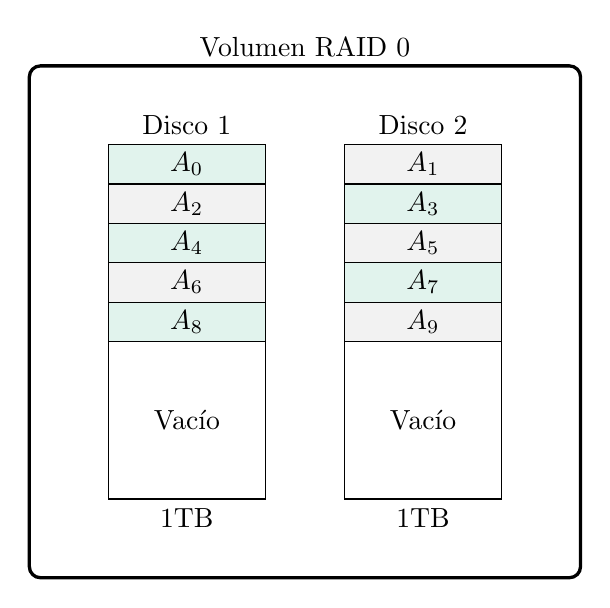
\begin{tikzpicture}
    \node[above] at (1,2.5) {Disco 1};
    \foreach \y\t\c in {
        0/8/white!95!blue!93!green,
        0.5/6/gray!10,
        1/4/white!95!blue!93!green,
        1.5/2/gray!10,
        2/0/white!95!blue!93!green}{
      \draw[fill=\c] (0,\y) rectangle node{\(A_\t\)} (2,{0.5+\y});
    }
    \draw (0,0) rectangle node{Vacío} (2,-2);
    \node[below] at (1,-2) {1TB};

    \node[above] at (4,2.5) {Disco 2};
    \foreach \y\t\c in {
        0/9/gray!10,
        0.5/7/white!95!blue!93!green,
        1/5/gray!10,
        1.5/3/white!95!blue!93!green,
        2/1/gray!10}{
      \draw[fill=\c] (3,\y) rectangle node{\(A_\t\)} (5,{0.5+\y});
    }
    \draw (3,0) rectangle node{Vacío} (5,-2);
    \node[below] at (4,-2) {1TB};

    \draw[very thick,rounded corners] (-1,-3) rectangle (6,3.5);
    \node[above] at (2.5,3.5) {Volumen RAID 0};
  \end{tikzpicture}
  \caption{Tamaño del volumen de RAID 0: 2TB.}
  \label{fig:raid0}
\end{figure}

Cuando se lee o escribe el archivo, ambos discos trabajan simultáneamente. Esto permite que la velocidad de transferencia sea considerablemente mayor que la de un solo disco, ya que las operaciones se realizan en paralelo.

\paragraph{Ventajas:}
\begin{itemize}
  \item Mayor velocidad de lectura y escritura.
  \item Se aprovecha el 100\% de la capacidad total de los discos.
  \item Implementación sencilla.
\end{itemize}

\paragraph{Desventajas:}
\begin{itemize}
  \item No proporciona redundancia ni tolerancia a fallos.
  \item Si falla un solo disco, se pierde toda la información del arreglo, porque cada archivo está repartido entre todos los discos.
\end{itemize}

\paragraph{Ejemplo}
Si se tienen dos discos de 1 TB, la capacidad total disponible es de 2 TB. Pero si uno de los discos deja de funcionar, el sistema pierde todos los archivos, ya que faltan partes de cada uno de ellos.

\begin{table}[!ht]
  \centering
  \begin{tabular}{l|c}
    Cantidad de discos mínima & 2 \\\hline
    Cantidad de discos que pueden fallar & 0 \\ \hline
    Velocidad de escritura relativa a un disco & \(N\times\)VDisco~[MB/s] \\\hline
    Velocidad de escritura ponderada & 10 \\ \hline
    Velocidad de lectura relativa a un disco & \(N\times\)VDisco~[MB/s] \\ \hline
    Velocidad de lectura ponderada & 10 \\ \hline
    Costo & Bajo
  \end{tabular}
  \caption{Características del RAID 0.}
\end{table}

\subsection{RAID 1}

RAID 1 es una técnica de almacenamiento cuyo objetivo principal es proporcionar redundancia y alta disponibilidad mediante espejado.

Conceptualmente, cada dato que se escribe en un disco se copia simultáneamente en otro disco. Ambos contienen exactamente la misma información, como se muestra en la figura \ref{fig:raid1}.

\begin{figure}[!ht]
  \centering
  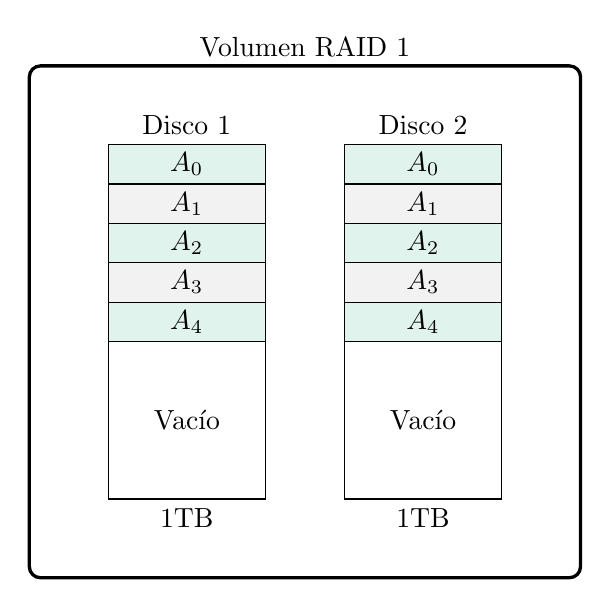
\begin{tikzpicture}
    \node[above] at (1,2.5) {Disco 1};
    \foreach \y\t\c in {
        0/4/white!95!blue!93!green,
        0.5/3/gray!10,
        1/2/white!95!blue!93!green,
        1.5/1/gray!10,
        2/0/white!95!blue!93!green}{
      \draw[fill=\c] (0,\y) rectangle node{\(A_\t\)} (2,{0.5+\y});
    }
    \draw (0,0) rectangle node{Vacío} (2,-2);
    \node[below] at (1,-2) {1TB};

    \node[above] at (4,2.5) {Disco 2};
    \foreach \y\t\c in {
        0/4/white!95!blue!93!green,
        0.5/3/gray!10,
        1/2/white!95!blue!93!green,
        1.5/1/gray!10,
        2/0/white!95!blue!93!green}{
      \draw[fill=\c] (3,\y) rectangle node{\(A_\t\)} (5,{0.5+\y});
    }
    \draw (3,0) rectangle node{Vacío} (5,-2);
    \node[below] at (4,-2) {1TB};

    \draw[very thick,rounded corners] (-1,-3) rectangle (6,3.5);
    \node[above] at (2.5,3.5) {Volumen RAID 1};
  \end{tikzpicture}
  \caption{Tamaño del volumen de RAID 1: 1TB.}
  \label{fig:raid1}
\end{figure}
Si uno de los discos falla, el otro sigue conteniendo una copia completa de todos los datos, por lo que el sistema puede continuar funcionando sin pérdida de información.

\paragraph{Ventajas:}
\begin{itemize}
  \item Alta tolerancia a fallos: soporta la falla de un disco (en un arreglo de dos discos).
  \item Recuperación sencilla: basta con reemplazar el disco averiado y reconstruir la copia.
  \item Las lecturas pueden ser más rápidas, ya que el sistema puede leer desde cualquiera de los discos.
\end{itemize}

\paragraph{Desventajas:}
\begin{itemize}
  \item La capacidad útil es solo la de un disco, ya que la otra mitad se utiliza para la copia.
  \item Las escrituras deben realizarse en todos los discos del espejo, por lo que el rendimiento de escritura no mejora significativamente.
\end{itemize}

\paragraph{Ejemplo}
Si se tienen dos discos de 1 TB la capacidad física total sigue siendo de 2 TB, pero la capacidad útil es de 1 TB. Sin embargo si uno de los discos falla, el sistema sigue funcionando con el otro disco y no se pierde información.

\subsubsection{RAID 1 + Hot Spare}

El Hot Spare (o disco de reserva en caliente) es un disco adicional que no almacena datos mientras el arreglo RAID funciona normalmente, sino que permanece disponible para reemplazar automáticamente a un disco que falle.

A modo de ejemplo, se supone un RAID 1 con dos discos y un Hot Spare, como se muestra en la figura \ref{fig:raid1spare}

\begin{figure}[!ht]
  \centering
  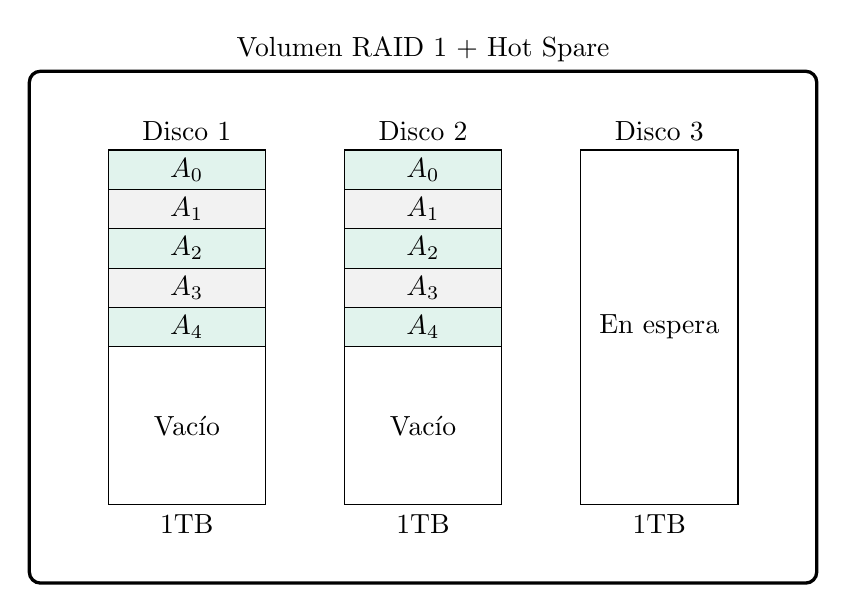
\begin{tikzpicture}
    \node[above] at (1,2.5) {Disco 1};
    \foreach \y\t\c in {
        0/4/white!95!blue!93!green,
        0.5/3/gray!10,
        1/2/white!95!blue!93!green,
        1.5/1/gray!10,
        2/0/white!95!blue!93!green}{
      \draw[fill=\c] (0,\y) rectangle node{\(A_\t\)} (2,{0.5+\y});
    }
    \draw (0,0) rectangle node{Vacío} (2,-2);
    \node[below] at (1,-2) {1TB};

    \node[above] at (4,2.5) {Disco 2};
    \foreach \y\t\c in {
        0/4/white!95!blue!93!green,
        0.5/3/gray!10,
        1/2/white!95!blue!93!green,
        1.5/1/gray!10,
        2/0/white!95!blue!93!green}{
      \draw[fill=\c] (3,\y) rectangle node{\(A_\t\)} (5,{0.5+\y});
    }
    \draw (3,0) rectangle node{Vacío} (5,-2);
    \node[below] at (4,-2) {1TB};

    \node[above] at (7,2.5) {Disco 3};
    \draw (6,2.5) rectangle node{En espera} (8,-2);
    \node[below] at (7,-2) {1TB};

    \draw[very thick,rounded corners] (-1,-3) rectangle (9,3.5);
    \node[above] at (4,3.5) {Volumen RAID 1 + Hot Spare};
  \end{tikzpicture}
  \caption{RAID 1 con Hot Spare. Tamaño final 1TB.}
  \label{fig:raid1spare}
\end{figure}

Si falla el Disco 1:
\begin{enumerate}
  \item El controlador RAID detecta la falla.
  \item Marca el Disco 1 como averiado.
  \item Incorpora automáticamente el Hot Spare al arreglo.
  \item Reconstruye los datos copiándolos desde el Disco 2 al Hot Spare.
\end{enumerate}
El resultado es:
\begin{itemize}
  \item Disco 1: Averiado
  \item Disco 2: Datos
  \item Disco 3: Nueva copia (antes era Hot Spare)
\end{itemize}
Una vez reemplazado físicamente el disco averiado, este puede configurarse como el nuevo Hot Spare.

\begin{table}[!ht]
  \centering
  \begin{tabular}{l|c}
    Cantidad de discos mínima & 2 \\\hline
    Cantidad de discos que pueden fallar & 1 \\ \hline
    Velocidad de escritura relativa a un disco & VDisco~[MB/s] \\\hline
    Velocidad de escritura ponderada & 5 \\ \hline
    Velocidad de lectura relativa a un disco & VDisco~[MB/s] \\ \hline
    Velocidad de lectura ponderada & 5 \\ \hline
    Costo & Medio
  \end{tabular}
  \caption{Características del RAID 1.}
\end{table}

\subsection{RAID 4}

RAID 4 combina el funcionamiento de RAID 0 a nivel de bloques, pero añade un disco adicional dedicado para almacenar la paridad, logrando un equilibrio entre rendimiento y tolerancia a fallos.

En este esquema, los datos se distribuyen entre varios discos, como en RAID 0, pero además existe un disco adicional que almacena información de paridad. La paridad permite reconstruir los datos de un disco si este falla.

Por ejemplo, con dos discos de datos y uno de paridad (Figura \ref{fig:raid4}):

\begin{figure}[!ht]
  \centering
  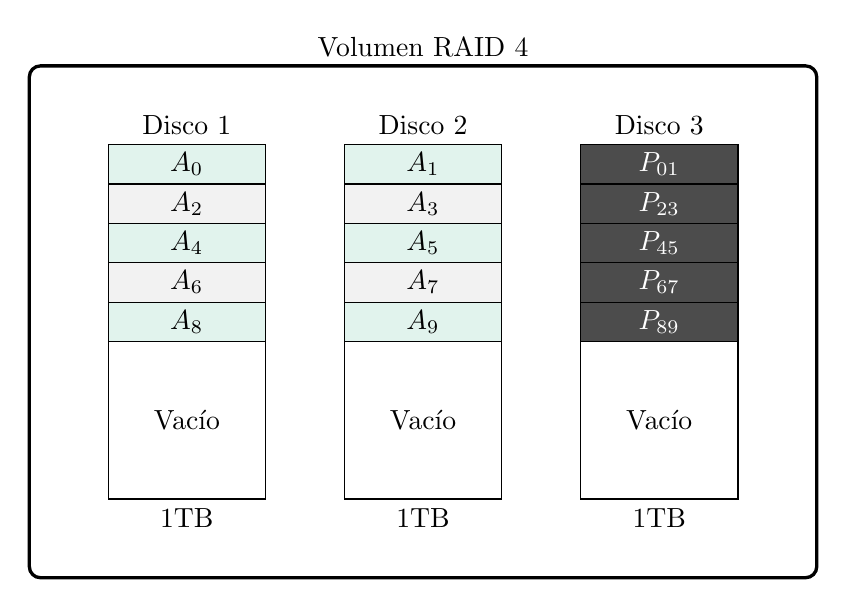
\begin{tikzpicture}
    \node[above] at (1,2.5) {Disco 1};
    \foreach \y\t\c in {
        0/8/white!95!blue!93!green,
        0.5/6/gray!10,
        1/4/white!95!blue!93!green,
        1.5/2/gray!10,
        2/0/white!95!blue!93!green}{
      \draw[fill=\c] (0,\y) rectangle node{\(A_\t\)} (2,{0.5+\y});
    }
    \draw (0,0) rectangle node{Vacío} (2,-2);
    \node[below] at (1,-2) {1TB};

    \node[above] at (4,2.5) {Disco 2};
    \foreach \y\t\c in {
        0/9/white!95!blue!93!green,
        0.5/7/gray!10,
        1/5/white!95!blue!93!green,
        1.5/3/gray!10,
        2/1/white!95!blue!93!green}{
      \draw[fill=\c] (3,\y) rectangle node{\(A_\t\)} (5,{0.5+\y});
    }
    \draw (3,0) rectangle node{Vacío} (5,-2);
    \node[below] at (4,-2) {1TB};

    \node[above] at (7,2.5) {Disco 3};
    \foreach \y\t in {
        0/89,
        0.5/67,
        1/45,
        1.5/23,
        2/01}{
      \draw[fill=black!70] (6,\y) rectangle node[white]{\(P_{\t}\)} (8,{0.5+\y});
    }
    \draw (6,0) rectangle node{Vacío} (8,-2);
    \node[below] at (7,-2) {1TB};

    \draw[very thick,rounded corners] (-1,-3) rectangle (9,3.5);
    \node[above] at (4,3.5) {Volumen RAID 4};
  \end{tikzpicture}
  \caption{Tamaño del volumen de RAID 4: 2TB.}
  \label{fig:raid4}
\end{figure}
Donde:
\begin{itemize}
  \item \(P_{01}\) es la paridad de los bloques \(A_0\) y \(A_1\),
  \item \(P_{23}\) es la paridad de los bloques \(A_2\) y \(A_3\),
  \item \(P_{45}\) es la paridad de los bloques \(A_4\) y \(A_5\) y así sucesivamente.
\end{itemize}
La paridad suele calcularse mediante la operación XOR:
\[
  P_{01} = A_0 \oplus A_1
\]
Si, por ejemplo, falla el Disco 2, el bloque perdido puede recuperarse usando:
\[
  A_1 = P_{01} \oplus A_0
\]
Y en caso de tener más de dos discos de datos, la paridad es simplemente la operación XOR entre todos los discos:
\[
  P = A_0 \oplus A_1 \oplus \cdots \oplus A_n
\]

\paragraph{Ventajas:}
\begin{itemize}
  \item Tolera la falla de un disco sin perder información.
  \item Las lecturas son rápidas, ya que los datos están distribuidos entre varios discos.
  \item Aprovecha mejor la capacidad que RAID 1.
\end{itemize}

\paragraph{Desventajas:}
\begin{itemize}
  \item Todas las escrituras deben actualizar el disco de paridad, lo que lo convierte en un cuello de botella.
  \item El rendimiento en escritura disminuye cuando hay muchas escrituras concurrentes.
\end{itemize}

\paragraph{¿Por qué RAID 4 casi no se utiliza?}

El principal problema es el disco de paridad dedicado. En cargas con muchas escrituras, ese disco debe actualizarse constantemente y termina limitando el rendimiento del arreglo o fallando por desgaste mecánico.

Por esta razón, en la práctica RAID 5 reemplazó casi por completo a RAID 4, ya que distribuye la paridad entre todos los discos y elimina la desventaja principal. RAID 4 se considera principalmente de interés histórico o académico.

\begin{table}[!ht]
  \centering
  \begin{tabular}{l|c}
    Cantidad de discos mínima & 3 \\\hline
    Cantidad de discos que pueden fallar & 1 \\ \hline
    Velocidad de escritura relativa a un disco & \(\frac{\text{VDisco}}{\text{Cant. Oper.}}\)~[MB/s] \\\hline
    Velocidad de escritura ponderada & 2 \\ \hline
    Velocidad de lectura relativa a un disco & VDisco~[MB/s] \\ \hline
    Velocidad de lectura ponderada & 5 \\ \hline
    Costo & Medio
  \end{tabular}
  \caption{Características del RAID 4.}
\end{table}

\subsection{RAID 5}

RAID 5 mejora la idea de RAID 4 al distribuir tanto los datos como la paridad entre todos los discos. De esta forma, elimina el cuello de botella que producía el disco de paridad dedicado.

Al igual que RAID 4, utiliza striping a nivel de bloques y almacena información de paridad para poder reconstruir los datos si un disco falla. La diferencia es que la paridad no se guarda siempre en el mismo disco, sino que rota entre todos ellos.

Por ejemplo, con tres discos (Figura \ref{fig:raid5}):
\begin{figure}[!ht]
  \centering
  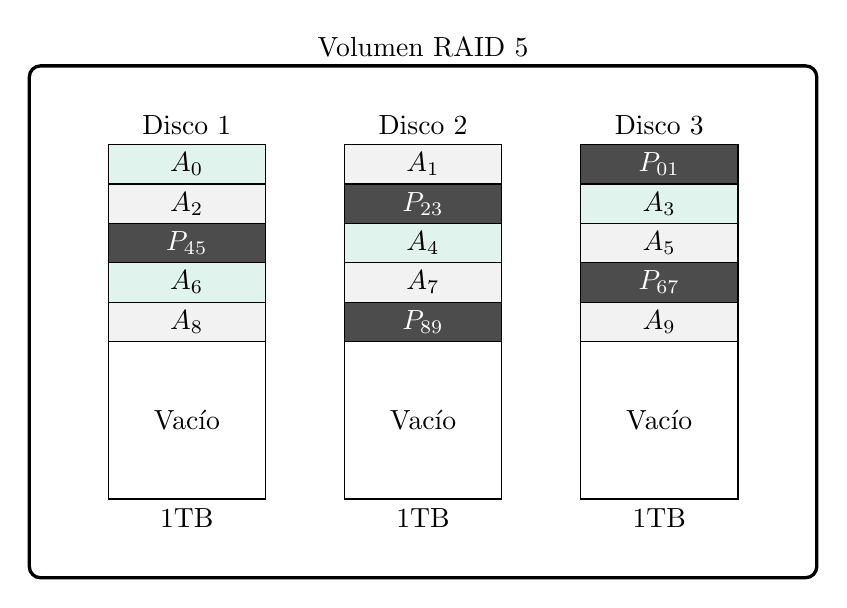
\begin{tikzpicture}
    \node[above] at (1,2.5) {Disco 1};
    \foreach \y\t\c in {
        0/A_8/gray!10,
        0.5/A_6/white!95!blue!93!green,
        1/\color{white}P_{45}/black!70,
        1.5/A_2/gray!10,
        2/A_0/white!95!blue!93!green}{
      \draw[fill=\c] (0,\y) rectangle node{\(\t\)} (2,{0.5+\y});
    }
    \draw (0,0) rectangle node{Vacío} (2,-2);
    \node[below] at (1,-2) {1TB};

    \node[above] at (4,2.5) {Disco 2};
    \foreach \y\t\c in {
        0/\color{white}P_{89}/black!70,
        0.5/A_7/gray!10,
        1/A_4/white!95!blue!93!green,
        1.5/\color{white}P_{23}/black!70,
        2/A_1/gray!10}{
      \draw[fill=\c] (3,\y) rectangle node{\(\t\)} (5,{0.5+\y});
    }
    \draw (3,0) rectangle node{Vacío} (5,-2);
    \node[below] at (4,-2) {1TB};

    \node[above] at (7,2.5) {Disco 3};
    \foreach \y\t\c in {
        0/A_9/gray!10,
        0.5/\color{white}P_{67}/black!70,
        1/A_5/gray!10,
        1.5/A_3/white!95!blue!93!green,
        2/\color{white}P_{01}/black!70}{
      \draw[fill=\c] (6,\y) rectangle node{\(\t\)} (8,{0.5+\y});
    }
    \draw (6,0) rectangle node{Vacío} (8,-2);
    \node[below] at (7,-2) {1TB};

    \draw[very thick,rounded corners] (-1,-3) rectangle (9,3.5);
    \node[above] at (4,3.5) {Volumen RAID 5};
  \end{tikzpicture}
  \caption{Tamaño del volumen de RAID 5: 2TB.}
  \label{fig:raid5}
\end{figure}
Cada fila contiene bloques de datos y un bloque de paridad, de forma similar a RAID 4, pero la paridad se almacena de forma alternada entre los discos disponibles. Al igual que RAID 4, la paridad se calcula mediante la operación XOR entre los datos.

Si falla un disco, el bloque faltante puede reconstruirse aplicando nuevamente XOR sobre los bloques restantes y la paridad.

\paragraph{Ventajas:}
\begin{itemize}
  \item Tolera la falla de un disco.
  \item No existe un único disco de paridad que limite el rendimiento o sufra mayor estrés mecánico.
  \item Excelente aprovechamiento del espacio: solo se pierde la capacidad equivalente a un disco para almacenar la paridad.
  \item Buen rendimiento en lectura.
\end{itemize}

\paragraph{Desventajas:}
\begin{itemize}
  \item Las escrituras son más lentas que en RAID 0, porque requieren recalcular y actualizar la paridad.
  \item La reconstrucción tras la falla de un disco puede ser lenta y exige mucho trabajo a los discos restantes.
\end{itemize}

\paragraph{Velocidad de Escritura}
Generalmente depende de la controladora, ya que al igual que RAID 4 requiere calcular la paridad entre los datos del Disco 1 y el Disco 2. A modo de ejemplo si se tiene \(A_0\) y se inserta \(A_1\), una escritura tendrá las siguientes cuatro operaciones:
\begin{enumerate}
  \item Escribir \(A_1\)
  \item Leer \(A_0\)
  \item Calcular \(P_{01}=A_0\oplus A_1\)
  \item Escribir \(P_{01}\)
\end{enumerate}

De este modo, si se supone la velocidad del Disco igual a 100~MB/s, resulta que 
\[
  \text{Velocidad de escritura relativa a un disco} = \frac{100~\text{MB/s}}{4} = 25~\text{MB/s}
\]

\begin{table}[!ht]
  \centering
  \begin{tabular}{l|c}
    Cantidad de discos mínima & 3 \\\hline
    Cantidad de discos que pueden fallar & 1 \\ \hline
    Velocidad de escritura relativa a un disco & \(\frac{\text{VDisco}}{\text{Cant. Oper.}}\)~[MB/s] \\\hline
    Velocidad de escritura ponderada & 2 \\ \hline
    Velocidad de lectura relativa a un disco & VDisco~[MB/s] \\ \hline
    Velocidad de lectura ponderada & 5 \\ \hline
    Costo & Medio
  \end{tabular}
  \caption{Características del RAID 5.}
\end{table}

\paragraph{Ejemplo}
Con cuatro discos de 1 TB:
\begin{itemize}
  \item Capacidad física total: 4 TB.
  \item Capacidad útil: 3 TB (la capacidad equivalente a un disco se destina a la paridad, aunque esté distribuida).
  \item Puede fallar un disco sin pérdida de datos.
\end{itemize}

\subsection{RAID 6}

RAID 6 es una extensión de RAID 5 que incorpora doble paridad distribuida. Su principal objetivo es aumentar la tolerancia a fallos, permitiendo que el arreglo continúe funcionando incluso si fallan simultáneamente dos discos.

Al igual que RAID 5, los datos se distribuyen mediante striping a nivel de bloques, pero cada conjunto de datos genera dos bloques de paridad independientes, que también se distribuyen entre todos los discos.

Un ejemplo conceptual con cuatro discos se muestra en la figura \ref{fig:raid6}.

\begin{figure}[!ht]
  \centering
  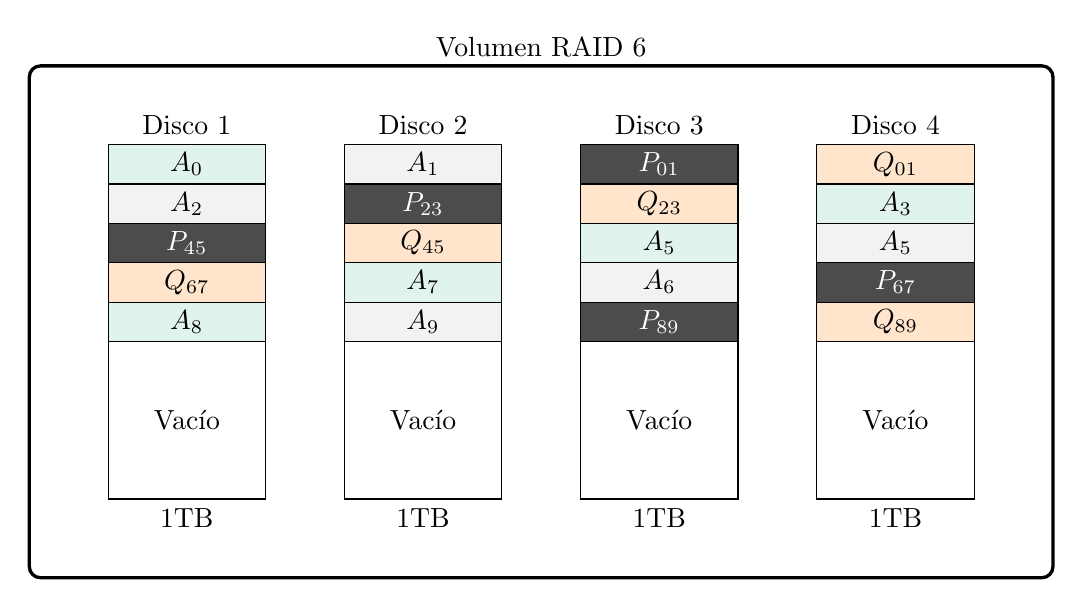
\begin{tikzpicture}
    \node[above] at (1,2.5) {Disco 1};
    \foreach \y\t\c in {
        0/A_8/white!95!blue!93!green,
        0.5/Q_{67}/orange!20,
        1/\color{white}P_{45}/black!70,
        1.5/A_2/gray!10,
        2/A_0/white!95!blue!93!green}{
      \draw[fill=\c] (0,\y) rectangle node{\(\t\)} (2,{0.5+\y});
    }
    \draw (0,0) rectangle node{Vacío} (2,-2);
    \node[below] at (1,-2) {1TB};

    \node[above] at (4,2.5) {Disco 2};
    \foreach \y\t\c in {
        0/A_9/gray!10,
        0.5/A_7/white!95!blue!93!green,
        1/Q_{45}/orange!20,
        1.5/\color{white}P_{23}/black!70,
        2/A_1/gray!10}{
      \draw[fill=\c] (3,\y) rectangle node{\(\t\)} (5,{0.5+\y});
    }
    \draw (3,0) rectangle node{Vacío} (5,-2);
    \node[below] at (4,-2) {1TB};

    \node[above] at (7,2.5) {Disco 3};
    \foreach \y\t\c in {
        0/\color{white}P_{89}/black!70,
        0.5/A_6/gray!10,
        1/A_5/white!95!blue!93!green,
        1.5/Q_{23}/orange!20,
        2/\color{white}P_{01}/black!70}{
      \draw[fill=\c] (6,\y) rectangle node{\(\t\)} (8,{0.5+\y});
    }
    \draw (6,0) rectangle node{Vacío} (8,-2);
    \node[below] at (7,-2) {1TB};

    \node[above] at (10,2.5) {Disco 4};
    \foreach \y\t\c in {
        0/Q_{89}/orange!20,
        0.5/\color{white}P_{67}/black!70,
        1/A_5/gray!10,
        1.5/A_3/white!95!blue!93!green,
        2/Q_{01}/orange!20}{
      \draw[fill=\c] (9,\y) rectangle node{\(\t\)} (11,{0.5+\y});
    }
    \draw (9,0) rectangle node{Vacío} (11,-2);
    \node[below] at (10,-2) {1TB};

    \draw[very thick,rounded corners] (-1,-3) rectangle (12,3.5);
    \node[above] at (5.5,3.5) {Volumen RAID 6};
  \end{tikzpicture}
  \caption{Tamaño del volumen de RAID 6: 2TB.}
  \label{fig:raid6}
\end{figure}

Donde:
\begin{itemize}
  \item P representa la primera paridad.
  \item Q representa la segunda paridad.
  \item Ambas se distribuyen entre todos los discos.
\end{itemize}
A diferencia de RAID 5, donde la paridad suele calcularse mediante una operación XOR, RAID 6 utiliza dos algoritmos de paridad distintos (uno de ellos suele ser XOR y el otro se basa en códigos de corrección, como Reed--Solomon). Gracias a ello, es posible recuperar la información incluso cuando se pierden los datos de dos discos.

\paragraph{Ventajas:}
\begin{itemize}
  \item Tolera la falla simultánea de dos discos.
  \item Muy alta disponibilidad y seguridad de los datos.
  \item La paridad está distribuida, por lo que no existe un disco dedicado que limite el rendimiento.
\end{itemize}

\paragraph{Desventajas:}
\begin{itemize}
  \item Las escrituras son más lentas que en RAID 5, ya que deben calcularse y actualizarse dos paridades.
  \item Requiere al menos cuatro discos.
  \item La implementación es más compleja.
\end{itemize}

\paragraph{Velocidad de Escritura}
Al igual que con RAID 5, depende de la controladora RAID, ya que requiere calcular dos paridades entre los datos del Disco de datos 1 y el Disco de datos 2. A modo de ejemplo si se tiene \(A_0\) y se inserta \(A_1\), una escritura tendrá las siguientes cuatro operaciones:
\begin{enumerate}
  \item Escribir \(A_1\)
  \item Leer \(A_0\)
  \item Calcular \(P_{01}\)
  \item Escribir \(P_{01}\)
  \item Calcular \(Q_{01}\)
  \item Escribir \(Q_{01}\)
\end{enumerate}

De este modo, si se supone la velocidad del Disco igual a 100~MB/s, resulta que 
\[
  \text{Velocidad de escritura relativa a un disco} = \frac{100~\text{MB/s}}{6} = 16.6~\text{MB/s}
\]

\begin{table}[!ht]
  \centering
  \begin{tabular}{l|c}
    Cantidad de discos mínima & 4 \\\hline
    Cantidad de discos que pueden fallar & 2 \\ \hline
    Velocidad de escritura relativa a un disco & \(\frac{\text{VDisco}}{\text{Cant. Oper.}}\)~[MB/s] \\\hline
    Velocidad de escritura ponderada & 2 \\ \hline
    Velocidad de lectura relativa a un disco & VDisco~[MB/s] \\ \hline
    Velocidad de lectura ponderada & 5 \\ \hline
    Costo & Alto
  \end{tabular}
  \caption{Características del RAID 6.}
\end{table}

\paragraph{Ejemplo}
Con seis discos de 1 TB:
\begin{itemize}
  \item Capacidad física total: 6 TB.
  \item Capacidad útil: 4 TB (la capacidad equivalente a dos discos se utiliza para la doble paridad).
  \item El sistema puede soportar la falla de dos discos sin perder información.
\end{itemize}
